\section{Internal SAGE sharing under stronger references}\label{sec:internal-sage}
This study examines whether a shared bank produces better combined predictions than capable single models and complete ensembles. It extends factor placement into the native SAGE stack and evaluates the resulting training procedures on encountered WikiCS development. It is separate from the original five-dataset benchmark and the Roman component study.

The internal version places input and output factor vectors around every native dense map, including the input/output projectors, SAGE projections and feed-forward maps. Shared matrices and native biases remain trainable and retain their original initialization; private factor vectors distinguish four routes. The first input factors start with independent signs, and later factors start at one. Each route receives its own persistent dropout stream and makes a complete native graph pass. Unlike the original boundary projectors in Section~\ref{sec:method}, this version retains the shared native bias and also changes the internal maps. Factor placement, initialization and bias are therefore distinct parts of the recipe.

The fixed configuration uses two residual SAGE blocks, hidden width 128, LayerNorm, dropout 0.2 and AdamW with learning rate 0.001 and zero decay. Training minimizes mean ordinary member cross-entropy, with no pooled-loss gradient or context auxiliary. Prediction averages member class probabilities. Checkpoints maximize pooled development accuracy, retaining the earliest strict maximum, with a 1,000-update ceiling and 300-update stale patience.

The matched joint untied bank gives each route a complete private body. Its initial route functions, factor/dropout starts, mean-member objective and coherent pooled checkpoint selection match the shared bank. The genuine factorized independent ensemble has four complete bodies with separate native starts, optimizers, unscaled own losses and own checkpoint selectors, followed by probability averaging. Ordinary and factorized singles retain their own full losses and selectors. These five arms compare complete acquisition procedures; their parameter ownership and optimization histories differ.

All results below are means over three paired optimizer seeds on the same 5,274 development nodes used for checkpoint selection. Fixed five-fold temperature calibration follows native selection. These selected development readouts do not provide unused whole-pipeline confirmation.

Figure~\ref{fig:internal-members-coverage} shows all five arms; Appendix Table~\ref{tab:internal-sage-F} gives their absolute scores and confidence metrics. The shared bank gains 0.720516 percentage points over matched joint untied4 and 0.537227 points over genuine factorized I4, with positive differences at every seed. It also gains 1.301985 points over the ordinary single and 1.491594 over the factorized single. The frozen raw accuracy screens pass. Descriptive paired-seed 95\% intervals are $[0.2712,1.1698]$ points versus joint untied4 and $[-0.2653,1.3398]$ versus I4; they condition on this setting and do not account for selection or variability across graphs.

\begin{figure}[t]
\centering
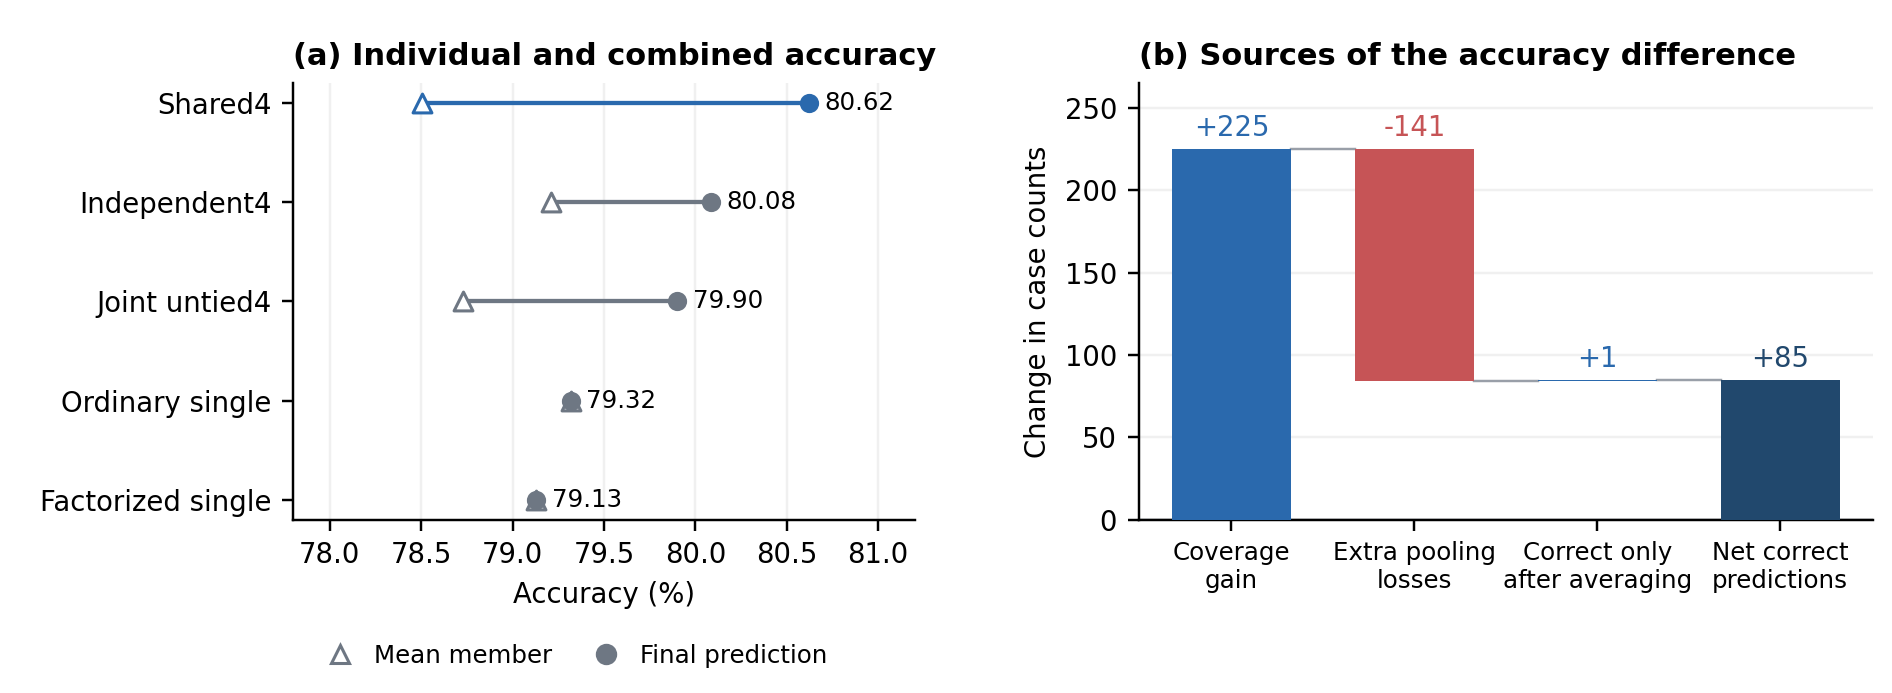
\includegraphics[width=\linewidth]{F_member_coverage_v2.png}
\caption{Internal SAGE on selected WikiCS development. (a) Shared4's average member is weaker than either complete ensemble control, while its combined prediction is more accurate. Both single-model references are shown. (b) Against independently acquired factorized models, 225 added covered cases are offset by 141 extra losses during averaging; one aggregation-only correction leaves 85 more correct decisions. Counts repeat the same 5,274 nodes across three optimizer seeds. The paired mean accuracy gain is 0.537 points, with a descriptive 95\% interval of $[-0.265,1.340]$; this is not unused confirmation or a statistically established superiority claim. Mean calibrated NLL harm is 0.021448, above the frozen 0.02 allowance.}
\label{fig:internal-members-coverage}
\end{figure}


The confidence protection does not fully pass. Mean calibrated NLL harm to I4 is 0.021448, above the frozen 0.02 allowance, although all three seed harms are below 0.05. The corresponding mean harm to joint untied4 is 0.013310 and passes. Thus the complete accuracy-and-confidence conjunction fails one condition. Calibrated Brier favors Shared4 over both ensemble controls, but does not replace the declared NLL rule. The result combines higher accuracy with a failed confidence-protection condition.

Coverage counts nodes with at least one correct member. A covered alternative can still be lost when the member probabilities are averaged. Across the three repeated readouts, Shared4 covers 13,731 cases versus 13,447 for joint untied4 and 13,506 for I4. It loses 976 of its covered cases in pooling, versus 805 and 835 for those controls. Shared4 also supplies one aggregation-only correction, leaving 114 and 85 more correct pooled decisions, respectively. Direct paired repairs/harms are 671/557 versus joint untied4 and 645/560 versus I4.

Shared4's members are less accurate on average than either ensemble control, yet the served bank is more accurate. This differs from the matched Roman SAGE result, where stronger members account for the gain. The two observations support reporting member quality and useful alternatives together. Their repeated-node counts are descriptive; they do not identify error covariance or establish a general cause of the learned differences.

Fewer stored weights remain a secondary benefit: Shared4 has 216,674 parameters, versus 832,256 for the complete four-body controls. Its recorded acquisition sum is 71.676 seconds, versus 50.025 for joint untied4 and 58.620 for I4. These scopes include different stopping histories and do not establish lower latency. Full seed, confidence, error and cost records accompany the study.

